\documentclass{./assets/wfis}
\usepackage[utf8]{inputenc}
\usepackage{amsmath}
\usepackage{tabularx}
\usepackage[hidelinks]{hyperref}
\usepackage{afterpage}
\usepackage{biblatex} 
\addbibresource{assets/references.bib}

\usepackage{framed}
\usepackage{listings}
\usepackage[most]{tcolorbox}
\usepackage{hyphenat}
% \usepackage[inkscapeformat=png]{svg}
\usepackage[inkscapelatex=false]{svg}
\begin{document}

\tytul{Wykrywanie zmian stanu skupienia przy użyciu aparatu EEG}
\autor{Mateusz Kojro}
\nralbumu{389105}
\promotor{dr hab. Krzysztofa Wardy}
\katedra{Teorii Ciała Stałego}
\kierunek{informatyka}
\specjalnosc{informatyka stosowana}
\typpracy{inżynierska}
\specjalizacja{Algorytmy i Programowanie}


\stronatytulowa

\begin{abstract}
W związku z ostatnimi postępami na pograniczu dziedzin neurologii i informatyki celem niniejszej pracy jest przygotowanie rozwiązania pozwalającego na wykrywanie zmian w poziomie skupienia badanej osoby za pomocą aparatu EEG (Elektroencefalografia).

W ramach projektu przygotowane zostaną następujące narzędzia pozwalające na przeprowadzenie badań, polegających na mierzeniu zmian potencjałów bioelektrycznych na skórze głowy ochotnika, w reakcji na bodziec wyświetlany na ekranie komputera:

\begin{itemize}
    \item Sterownik układu EEG, program działający na mikrokomputerze Raspberry PI pozwalający na odczytywanie, interpretowanie oraz zapisywanie informacji zbieranych przez układ czujników.
    \item Generator bodźca, strona internetowa pozwalająca na wyświetlanie pytań, zapisywanie udzielonych odpowiedzi oraz korelowanie ich w czasie z uzyskanymi pomiarami.
\end{itemize}

Wyniki przeprowadzonych badań zostaną następnie wykorzystane do przygotowania modelu informatycznego, opierającego się na algorytmach uczenia maszynowego, pozwalającego na wykrywanie zmian w poziomie skupienia.
\end{abstract}

\chapter{Wstęp}
\section{Basic opis - cel}
\section{Other Work}

\chapter{Podstawy teoretyczne}

\section{EEG}
Elektroencefalografia (EEG) to badanie polegające na pomiarze względnych potencjałów elektrycznych na czaszce pacjenta za pomocą różnego rodzaju elektrod. Zebrane w ten sposób informacje pozwalają na określenie względnej aktywności różnych obszarów mózgu w porównaniu do wartości obserwowanych u zdrowej osoby lub w relacji na bodziec (np. zamknięcie oczu).

Elektroencefalografia tradycyjnie wykorzystywana jest między innymi do diagnozowania schorzeń neurologicznych takich jak epilepsja, nowotwory mózgu czy zaburzenia snu. Podczas badania, operator wizualnie analizuje wykresy sygnałów o różnych częstotliwościach w czasie. W związku z relatywnie niskim poziomem sygnału do szumu oraz skomplikowanymi relacjami ukrytymi w wynikach oraz łatwy dostęp do aparatury pomiarowej pozwalający na stosunkowo proste zbieranie znaczących ilości danych rozpoczęto prace nad zastosowaniem algorytmów uczenia maszynowego w celu diagnozy innych jednostek chorobowych takich jak ADHD, dysleksja czy schizofrenia \cite{ahire_comprehensive_2022, joshi_review_2021, clarke_eeg_2002}.

\subsection{Mechanizm Działania}
% Potencjał czynnościowy (ang. \textit{action potential}) zmienia wewnętrzne napięcie neuronu o $\approx100mV$ na czas około $3ms$, biorąc pod uwagę odległość elektrod od źródła sygnału (natężenie pola elektrycznego spada z kwadratem odległości) oraz właściwości tłumiące tkanek ludzkich, pomiar aktywności pojedynczych neuronów za pomocą elektrod umieszczonych na skórze głowy jest niemożliwe.

Układ nerwowy człowieka przekazuje oraz przetwarza informacje za pomocą impulsów elektrycznych (potencjałów czynnościowych) wytwarzanych w komórkach nerwowych (neuronach), z pomocą mechanizmu xxxxx. Ze względu na dużą liczbę neuronów w ludzkim mózgu ($\approx10^9$\cite{herculano-houzel_human_2009}), ich małe rozmiary (xxxx) małe napięcie impulsu potencjału czynnościowego ($\approx100mV$\cite{biga_125_2019}) oraz krótki czas jego trwania ($\approx2ms$\cite{biga_125_2019}) niemożliwe jest badanie pracy pojedynczych neuronów, a jedynie średnich wartości milionów zsynchronizowanych impulsów na przestrzeni centymetrów (xxxxxx). Ograniczenia te powodują, że różne obszary mózgu mogą być badane z różną dokładnością (najlepszą sprawność otrzymuje się w rejonach mózgu znajdujących się blisko powierzchni skóry zawierających dużą liczbę tzw. neuronów piramidowych – np. kora przedczołowa).

\subsection{Metodyka Badania}

W zależności od specyfiki badania ważny jest dobór następujących parametrów:

\subsubsection{Rozmieszczenie elektrod}
Ogólnoprzyjętymi standardami pozycjonowania są tzw. międzynarodowe systemy $10$-$10$ i $10$-$20$ (przedstawiono na rysunku \ref{fig:10-20-system}), stosowanie tych metod pozwala na stosunkowo łatwe powielanie i porównywanie wyników badań przeprowadzonych w różnych placówkach. Alternatywnie 
% (nazewnictwo wywodzi się od procentowych podziałów czaszki – elektroda znajduje się co $10\%$ obwodu czaszki na osi przód – tył i co $20\%$ na osi prawo – lewo)

\begin{figure}[h]
    \centering
    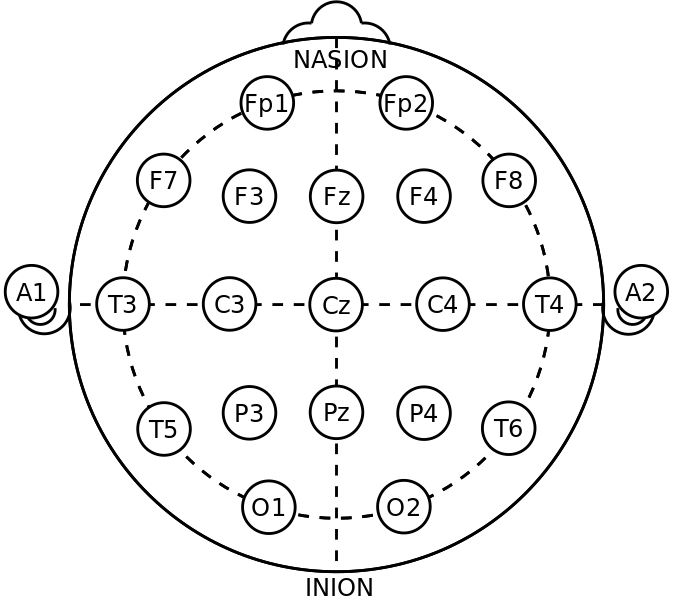
\includegraphics[width=0.5\columnwidth]{thesis/assets/10-20_system_electrodes.png}
    \caption{Rozmieszczenie elektrod w międzynarodowym systemie $10$-$20$}
    \label{fig:10-20-system}
\end{figure}

\subsubsection{Rodzaj elektrod}
Ze względu na jakość wyników, długość trwania badania oraz okoliczności towarzyszące badaniu konieczny jest dobór odpowiedniego typu elektrod. Najpopularniejsze z nich to:

\begin{itemize}
    \item \textbf{Elektrody żelowe} - Zapewniają wysoki poziom komfortu oraz dokładności pomiarów, wymagają aplikacji specjalnego żelu przewodzącego, utrudniając prowadzenie badań w warunkach terenowych.
    \item \textbf{Elektrody gąbkowe} - Pozwalają na kompromis pomiędzy jakością zebranych danych a łatwością aplikacji (żel przewodzący zamieniany jest na roztwór soli).
    \item \textbf{Elektrody suche} - Oferują najniższy poziom komfortu oraz dokładności, w zamian za bardzo wysoką łatwość użycia.
\end{itemize}

\subsubsection{Montaż}
Podczas badania EEG montażem nazywa się konfiguracje punktów odniesienia dla poszczególnych elektrod. Najbardziej popularnymi metodami montażu są:
% Some info in the summary of the book: https://docs.google.com/document/d/1bB9OZkO2m4fax8v3bGp_QZP7pAD-WryXQr4PxMppVp8/edit


\subsubsection{Badane częstotliwości}

\begin{table}[h]
    \centering
    \begin{tabular}{|c|c|c|}
        \hline
        Oznaczenie & Zakres częstotliwości & Zastosowanie \\
        \hline
        $\delta$ & $1$-$3Hz$ & \\
        $\theta$ & $4$-$7Hz$ & \\
        $\alpha$ & $8$-$12Hz$ & \\
        $\beta$  & $13$-$25Hz$ & \\
        $\gamma$ & $>25Hz$ & \\
        \hline
    \end{tabular}
    \caption{Typowe oznaczenia badanych częstotliwości}
    \label{tab:freqs}
\end{table}

\chapter{Metody}


\section{Aparatura Pomiarowa}
 W celu przeprowadzenia badan przygotowano aplikację webową pozwalającą na wyświetlanie bodźców na ekranie komputera oraz korelowanie ich w czasie z sygnałem EEG mierzonym za pomocą zakupionego urządzenia – \textit{Emotiv EPOCX}

\subsection{Strona internetowa}
\subsection{Zestaw Emotiv EpocX}\label{emotiv}

\section{Procedura przeprowadzonych badań}
\section{Architektury algorytmów uczenia maszynowego}
- sieci neuronowe
- random forest
- clustering algorithms


\chapter{Wyniki}
\section{Demografia}
- Wiek
- Płeć
- Wykształcenie
- Zawód
- Choroby neurologiczne/psychologiczne
- Stopien zaznajomienia z komputerami
\section{Confunding variables}
- Praca umsylowa danego dnia
- Poziom zmeczenia
- Otoczenie (miejscie zamieszkania obce znajome)
- Pora dnia
- Godziny snu poprzedniej nocy
- Uzywki (kawa, papierosy) w ciagu ostatnich 6h
\section{Standard analysys}
\subsection{ANOVA}
\section{Uczenie maszynowe}
\section{Bias analysys - Shaply values}

\chapter{Dyskusja}

\appendix
\chapter{Formularz dla osób badanych}
\chapter{Instrukcja uruchomienia i obsługi oprogramowania}

\printbibliography

\clearpage
\thispagestyle{empty}
\listoffigures
\listoftables
\clearpage

\end{document}